
\section{Разработка цифровой видеосистемы для дрона}

\subsection{Обзор цифровых видеосистем}

Цифровая видеосистема -- система передачи данных, использующая двунаправленный канал передачи данных с использованием цифрового кодирования сигнала. В сочетании со специальным программным обеспечением позволяет передавать видеосигнал высокого разрешения с минимальными задержками.

Существуют как готовые решения, так и проекты с открытым исходным кодом. Рассмотрим коммерческие продукты.

В 2021 году на рынке видеосистем наиболее популярны Connex ProSight HD, DJI FPV, Fat Shark SharkByte \cite{oscar} (рис. \ref{fig:HD}).
Их стоимость начинается с 250\$ за комплект, в который входят камера и  модули приема-передачи. 
Наземная система DJI FPV является видеошлемом со встроенным модулем приемо-передачи. Connex ProSight HD и Fat Shark SharkByte представляют собой отдельный наземный модуль, что является более дешевым и универсальным решением.

Помимо высокой стоимости можно отметить следующие недостатки:
\begin{itemize}
	\item Габаритность, вес камеры и бортового модуля в 25-50 г;
	\item Для DJI FPV в комплекте идет дорогостоящий шлем, который не нужен для выполнения моей задачи, а передача на станцию доступна только по HDMI проводу;
	\item А также закрытое программное обеспечение. 
\end{itemize}

\begin{figure}[H]
	\centering
	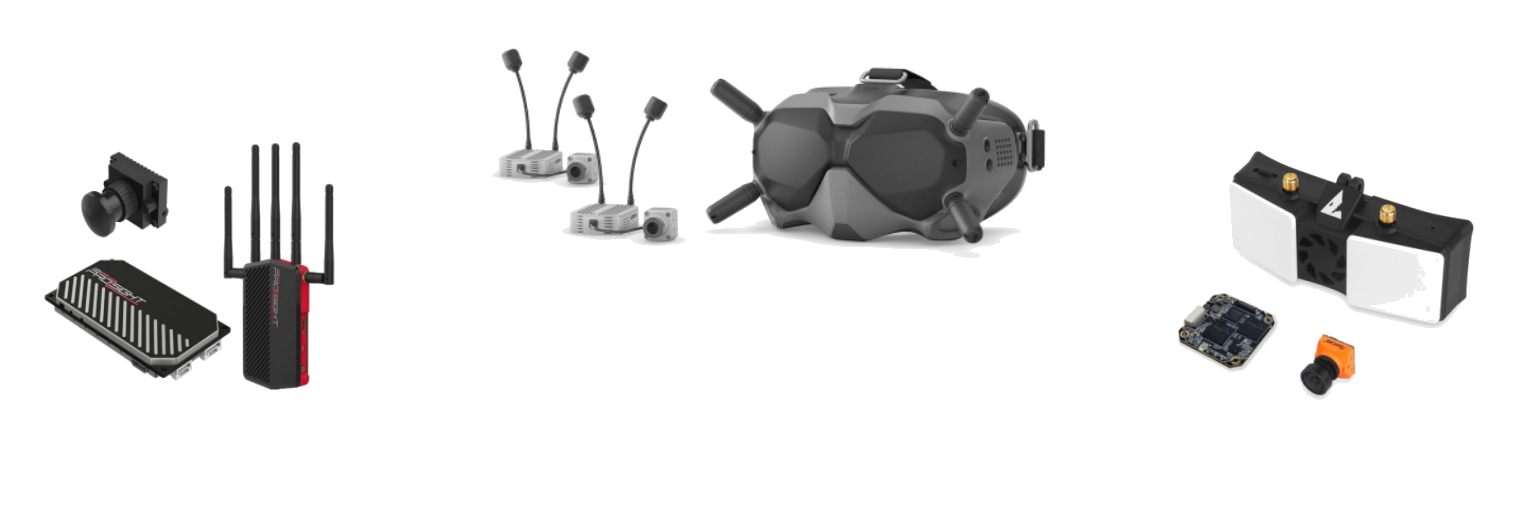
\includegraphics[width=0.7\linewidth]{pics/buyHD}
	\caption{ Connex ProSight HD, DJI FPV, Fat Shark SharkByte (слева направо) 
	}
	\label{fig:HD}
\end{figure}

Альтернативой коммерческим продуктам являются open-source и open-hardware решения, среди которых самые популярные -- EZ-Wi\-fi\-Broadcast и Open.HD.

EZ-WifiBroadcast -- это система передачи цифрового видеосигнала через Wi-Fi канал. В качестве аппаратной части используются одноплатные микрокомпьютеры Raspberry Pi (рис. \ref{fig:openhd}). При отсутствии встроенного Wi-Fi модуля в выбранной модели Raspberry или желании увеличить радиус действия сигнала используются внешние Wi-Fi модули. Программное обеспечение из репозитория проекта позволяет передавать HD-видео, данные телеметрии и управляющий сигнал между конечными точками с малой задержкой. При ухудшении сигнала EZ-WifiBroadcast пытается имитировать известные свойства аналогового соединения - помехи, в то время как в коммерческих решениях полностью пропадает изображение \cite{EZ}.

\begin{figure}[H]
	\centering
	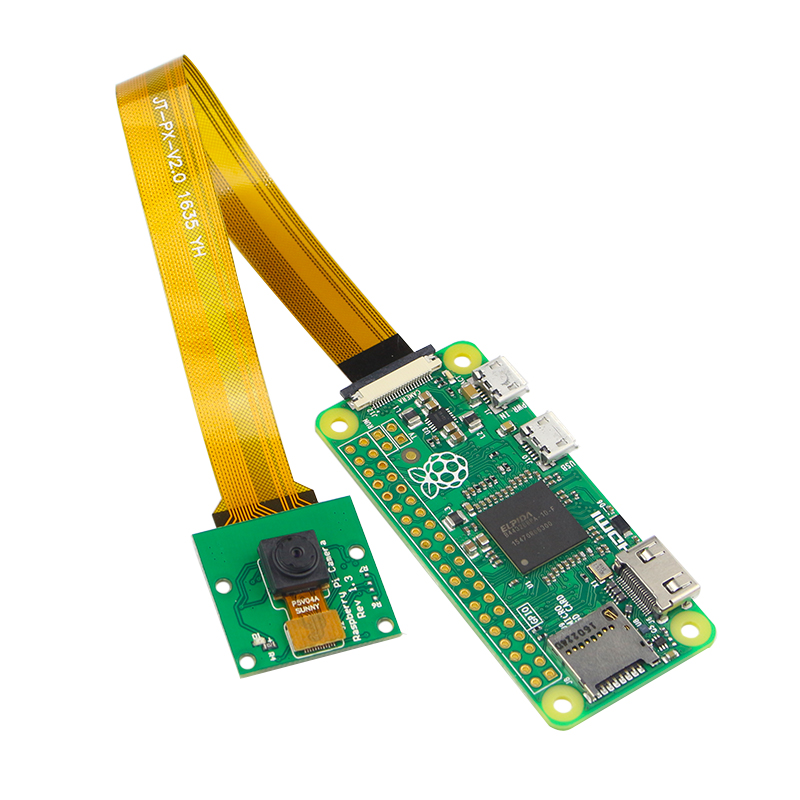
\includegraphics[width=0.5\linewidth]{pics/openhd}
	\caption{ Аппаратная бортовая часть БПЛА, используемая в Open.HD и EZ-WifiBroadcast
	}
	\label{fig:openhd}
\end{figure}

Ключевые особенности EZ-WifiBroadcast:
\begin{itemize}
	\item Поддержка Raspberry Pi1A+, Pi1B+, Pi2B, Pi3B, Pi Zero;
	\item Средняя задержка около 130 мс;
	\item Поддерживаются камеры Raspberry Pi V1 и V2;
	\item Максимальное разрешение изображения до 1920x1080p при 30 кадрах в секунду и скорость передачи видео до 12 Мбит;
	\item Поддержка диапазонов частоты 2,3 - 2,5 ГГц, а также диапазонов от 5,2 до 5,8 ГГц;
	\item Поддержка двунаправленной телеметрии по протоколу MAVLink;
	\item Радиоуправление через MAVLink, SUMD (Graupner / JR), IBUS (FlySky), SRXL (Multiplex);
	\item Включение и установка связи производится за 10 секунд.
\end{itemize}

Open.HD является форком EZ-WifiBroadcast, и имеет ряд преимуществ. Главным приоритетом проекта являются простота эксплуатации и стабильность работы. Стоит разобраться с данным проектом подробнее.

\subsection{Open.HD}
%https://github.com/OpenHD/Open.HD/wiki/General-~-Features

Возможности проекта:
\begin{itemize}
	\item Поддержка Raspberry Pi A+, Pi1B+, Pi2B, Pi3B, Pi3B+, Pi3A+, Pi4, Pi4B, Pi Zero, Pi Zero W, Odroid-W, Pi V1 и V2;
	\item Максимально возможные разрешения (в зависимости от используемой камеры): 1280x720p 60 кадров в секунду; 1296x972p 42 кадра в секунду; 1640x922p 40 кадров в секунду; 1920x1080p 30 кадров в секунду;
	\item Максимально возможный битрейт видео около 12Мбит;
	\item Задержка ~125 мс при настройках по умолчанию (720p при 48 кадрах в секунду), минимально возможная задержка около 110 мс;
	\item Поддержка диапазонов 2,3 - 2,5 ГГц и диапазонов от 5,2 до 5,8 ГГц;
	\item Перенаправление видеопотока и данных телеметрии на 2-й дисплей через: USB-модем, точку доступа Wi-Fi, Ethernet, режим ретрансляции Wifibroadcast;
	\item Поддержка двунаправленной телеметрии по протоколу MAVLink;
	\item Поддержка видео и телеметрии внутри QGroundcontrol, Mission Planner;
	\item Автоматическое обнаружение второго дисплея;
	\item Интегрированное настраиваемое экранное меню с поддержкой телеметрии MAVLink, Frsky, LTM, Smartport;
	\item Возможность записывать видео в формате AVI, делать снимки экрана в формате PNG и сохранять данные телеметрии на USB-накопитель;
	\item Автоматическое построение графиков RSSI, потерь пакетов, битрейта видео и других данных;
	\item Стабильный прием видео в сложных условия, как в аналоговом режиме;
	\item Зашифрованный радиосигнал;
	\item Наличие аудиозаписи;
	\item Настройки производятся через приложение для Android (часть проекта Open.HD);
	\item Возможность переключения частотного диапазона \cite{openhd}.
\end{itemize}

Перечисленные возможности отлично подходят под разрабатываемый комплекс.
Обобщенно устройство системы выглядит следующим образом: с помощью Wi-Fi модулей происходит обмен телеметрией между наземным (Ground\-Pi) и воздушным (AirPi) модулем, а также отправка радиосигнала и получение видео наземной станцией. Камера подключается к воздушному модулю по CSI (стандарт подключения камер). CSI максимально упрощает интеграцию камеры в систему; предварительная обработка изображения выполняется блоком обработки сигналов изображения процессора хост-системы, что позволяет проектировать встраиваемые системы с низким ресурсопотреблением без ущерба для качества изображения.

Для просмотра изображения с борта БПЛА к наземному модулю подключается монитор по DSI (стандарт подключения дисплеев, направленный на снижение затрат на дисплейную подсистему) или micro-HDMI. Воздушный модуль подключается к полетному контроллеру БПЛА по UART, и получает данные о состоянии дрона (напряжение батареи, токопотребление, время полета...) по протоколу MAVLink. Подключение к модулям доступно через SSH.

Блочная схема архитектуры решения представлена на рисунке \ref{fig:OpenHDSetup}.

\begin{figure}[H]
	\centering
	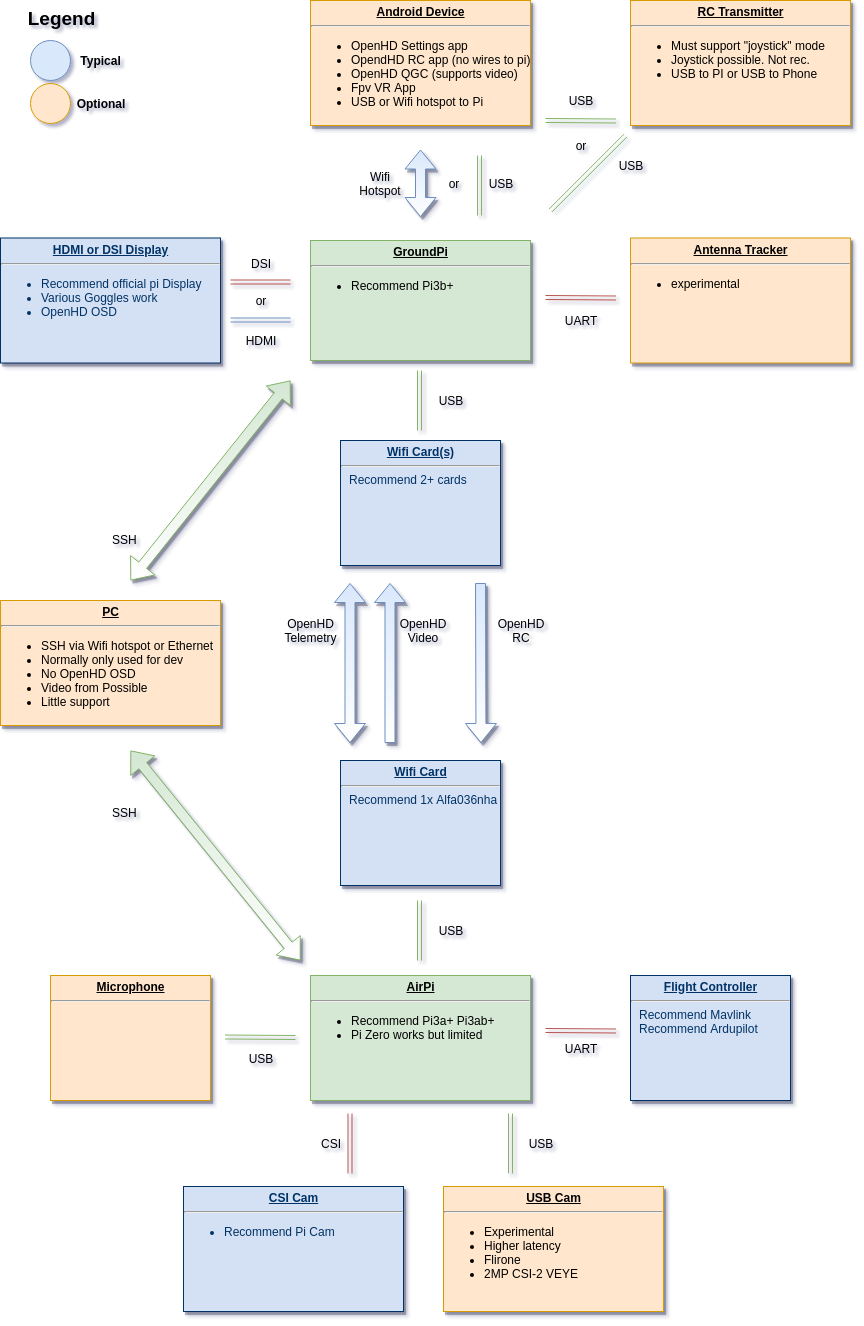
\includegraphics[width=0.8\linewidth]{pics/OpenHDSetup}
	\caption{ Архитектура проекта
	}
	\label{fig:OpenHDSetup}
\end{figure}

\subsection{Подготовка аппаратной части}
%https://github.com/OpenHD/Open.HD/wiki/Hardware-~-Proper-Wiring

Для экспериментальных образцов было решено использовать следующее оборудование (рис. \ref{fig:photo1}):
\begin{itemize}
	\item Raspberry Pi 4B;
	\item Raspberry Zero W;
	\item RPi Zero V1.3 Camera.
\end{itemize}

\begin{figure}[H]
	\centering
	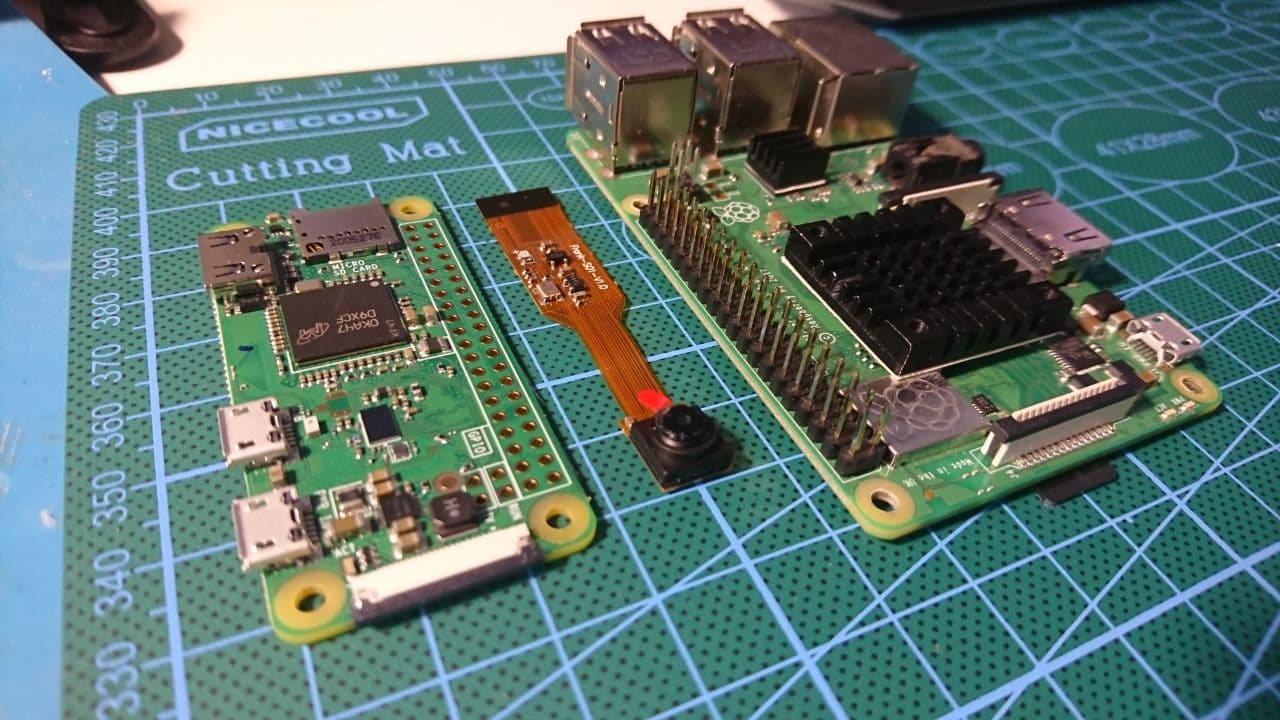
\includegraphics[width=0.5\linewidth]{pics/photo1}
	\caption{ Используемое оборудование
	}
	\label{fig:photo1}
\end{figure}

Оба микрокопьютера обладают встроенным Wi-Fi модулем, поддерживаются Open.HD, и имеют запас по ресурсам.
Raspberry Pi 4B будет использоваться в наземной станции. Его преимущества по сравнению с предыдущими поколениями:
\begin{itemize}
	 \item однокристальная система Broadcom BCM2711 -- кристалл включает в себя 4-ядерный 64-битный процессор Cortex-A72 (ARM v8) с частотой 1,5 ГГц и графический процессор GPU VideoCore VI с частотой 500 МГц ( по данным производителя, система на новой архитектуре стала на 50\% быстрее, чем прошлые поколения Raspberry Pi);
	\item Аппаратное ускорение видеопотока H.265;
	\item Наличие портов USB 3.0;
	\item Гигабитный контроллер Ethernet;
	\item Увеличенный объём ОЗУ (4Гб);
	\item Стандарты беспроводных модулей Wi-Fi 802.11 b/g/n/ac и протокол 
	\begin{otherlanguage}{english}
		Bluetooth
	\end{otherlanguage}
	5.0 с BLE.
\end{itemize}

RPi Zero V1.3 Camera -  камера размером 60*11.5*5 mm. Угол обзора 72 градуса, разрешение 5mpx. Максимальное разрешение составляет 1080p. Подключение к Raspberry Pi Zero W производится стандартным шлейфом к интерфейсу CSI. 

Питание Raspberry (GroundPi и AirPi) производится через bec'и на 5В 3А. Для фильтрации шумов по питанию рекомендуется использовать low ESR конденсаторы на входе. Чтобы исключить проблемы, связанные с питанием/соединением, используются провода не менее 20 AWG \cite{openhd}.

Далее необходимо загрузить образы на micro-SD карты и произвести конфигурацию системы.
\begin{figure}[H]
	\centering
	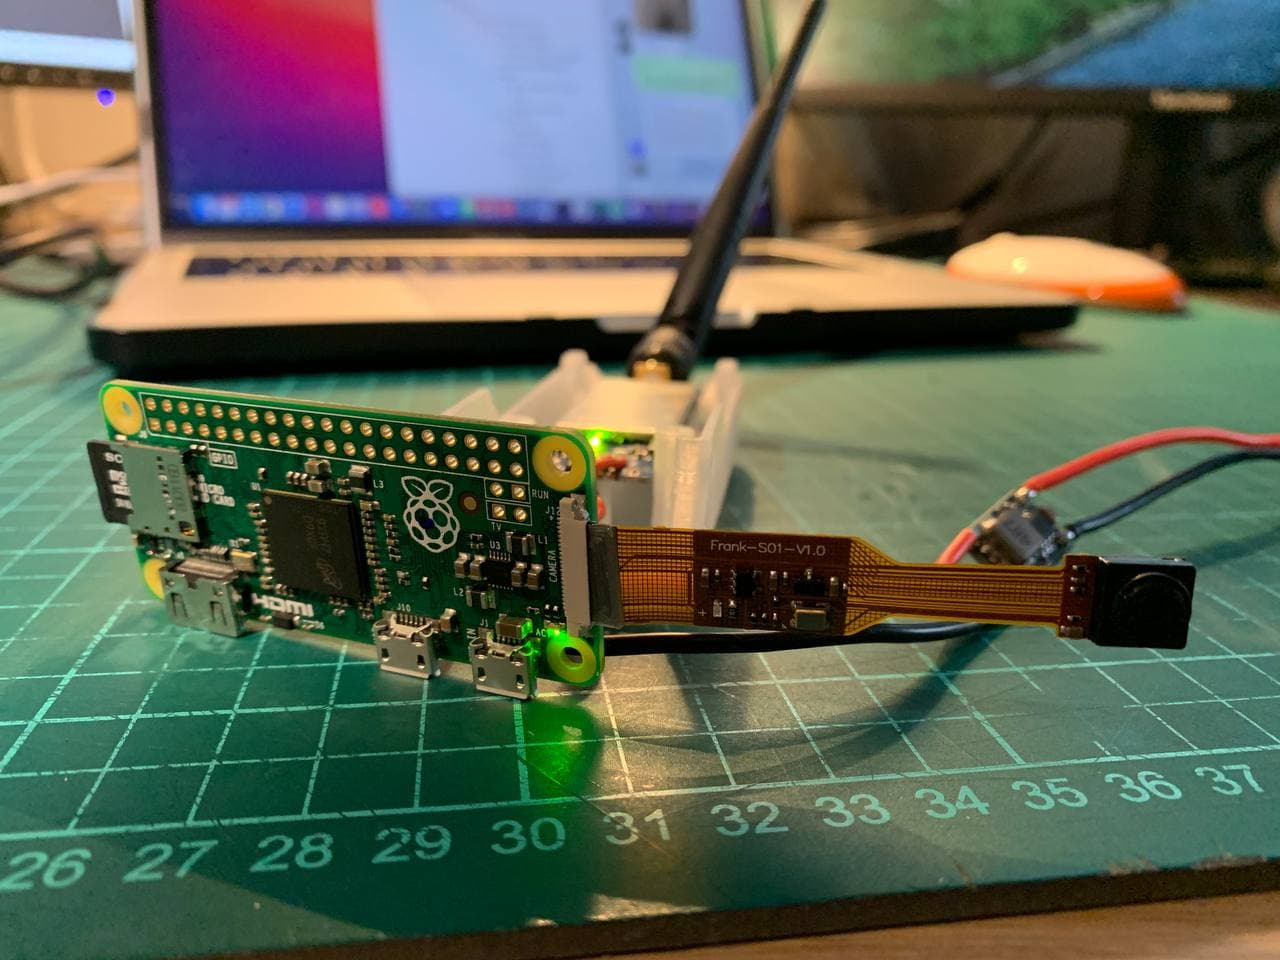
\includegraphics[width=0.5\linewidth]{pics/photo4}
	\caption{ Воздушный модуль в сборе
	}
	\label{fig:photo4}
\end{figure}

%\cite{manual}
\subsection{Настройка}

Для образов системы необходимы micro-SD карты объемом не менее 4 Гб. Со страницы релизов репозитория Open.HD необходимо скачать и распаковать  образы для AirPi и GroundPi. После этого записать их на соответствующие micro-SD. Описанные шаги выполняются с помощью команд, представленных в листинге \ref{lst:1}.

\begin{Program}[H]
	\caption{Команды для записи образов} \label{lst:1}
	\begin{MyCode}
$ wget https://release-openhdfpv.eu-central-1.linodeobjects.com/Open.HD-2.0.8-stretch.img.gz
$ gunzip Open.HD-2.0.8-stretch.img.gz
$ sudo fdisk -l
$ sudo umount /dev/sda
$ sudo dd if=~/Open.HD-2.0.8-buster.img.gz of=/dev/sda
$ sync
	\end{MyCode}
\end{Program}

После установки карт в микрокомпьютеры и подачи питания происходит загрузка и установка соединения системы. Первоначальное тестирование системы будет производиться на настройках по умолчанию. После получения результатов будет проведен анализ, какие настройки необходимо изменить.


